\chapter{Le Grand collisionneur de hadrons (LHC)}
\renewcommand\chapterillustration{LHC/lhc}
\ThisULCornerWallPaper{1}{\chapterillustration}
\minitoc
\vspace{1cm}
\lettrines{C}{e} chapitre décrit le complexe des accélérateurs du CERN\footnote{Organisation Européenne pour le Recherche Nucléaire} qui permet d'accélérer les particules, afin d'avoir un faisceau de particule avec une énergie suffisante (7 TeV) pour être injecter dans le Grand collisionneur de hadrons (LHC\footnote{Large Hadron Collider}). Cette déscription bien que succinte est nécessaire car de nombreux résultats obtenus durant cette thèse ont nécessité l'utilisation d'accélérateur de ce complexe. Une description du LHC est également donnée, car ses performances présentes et futurs déterminent les choix technologiques des détecteurs utilisant son faisceau.

\section{Le complexe d'accélérateur du CERN}
Le complexe d'accélérateur (\ref{complexe}) du CERN est une série de machines qui délivrent des faisceaux de particules (p $P_{b}$) d'énergies de plus en plus élevés. Chaque machine accélère les faisceaux et les injecte dans la machine suivante. Le dernier accélérateur du complexe, le Large Hadron Collider amène les faisceaux à une énergie de 7 TeV.
\begin{figure}[h]
	\centering
  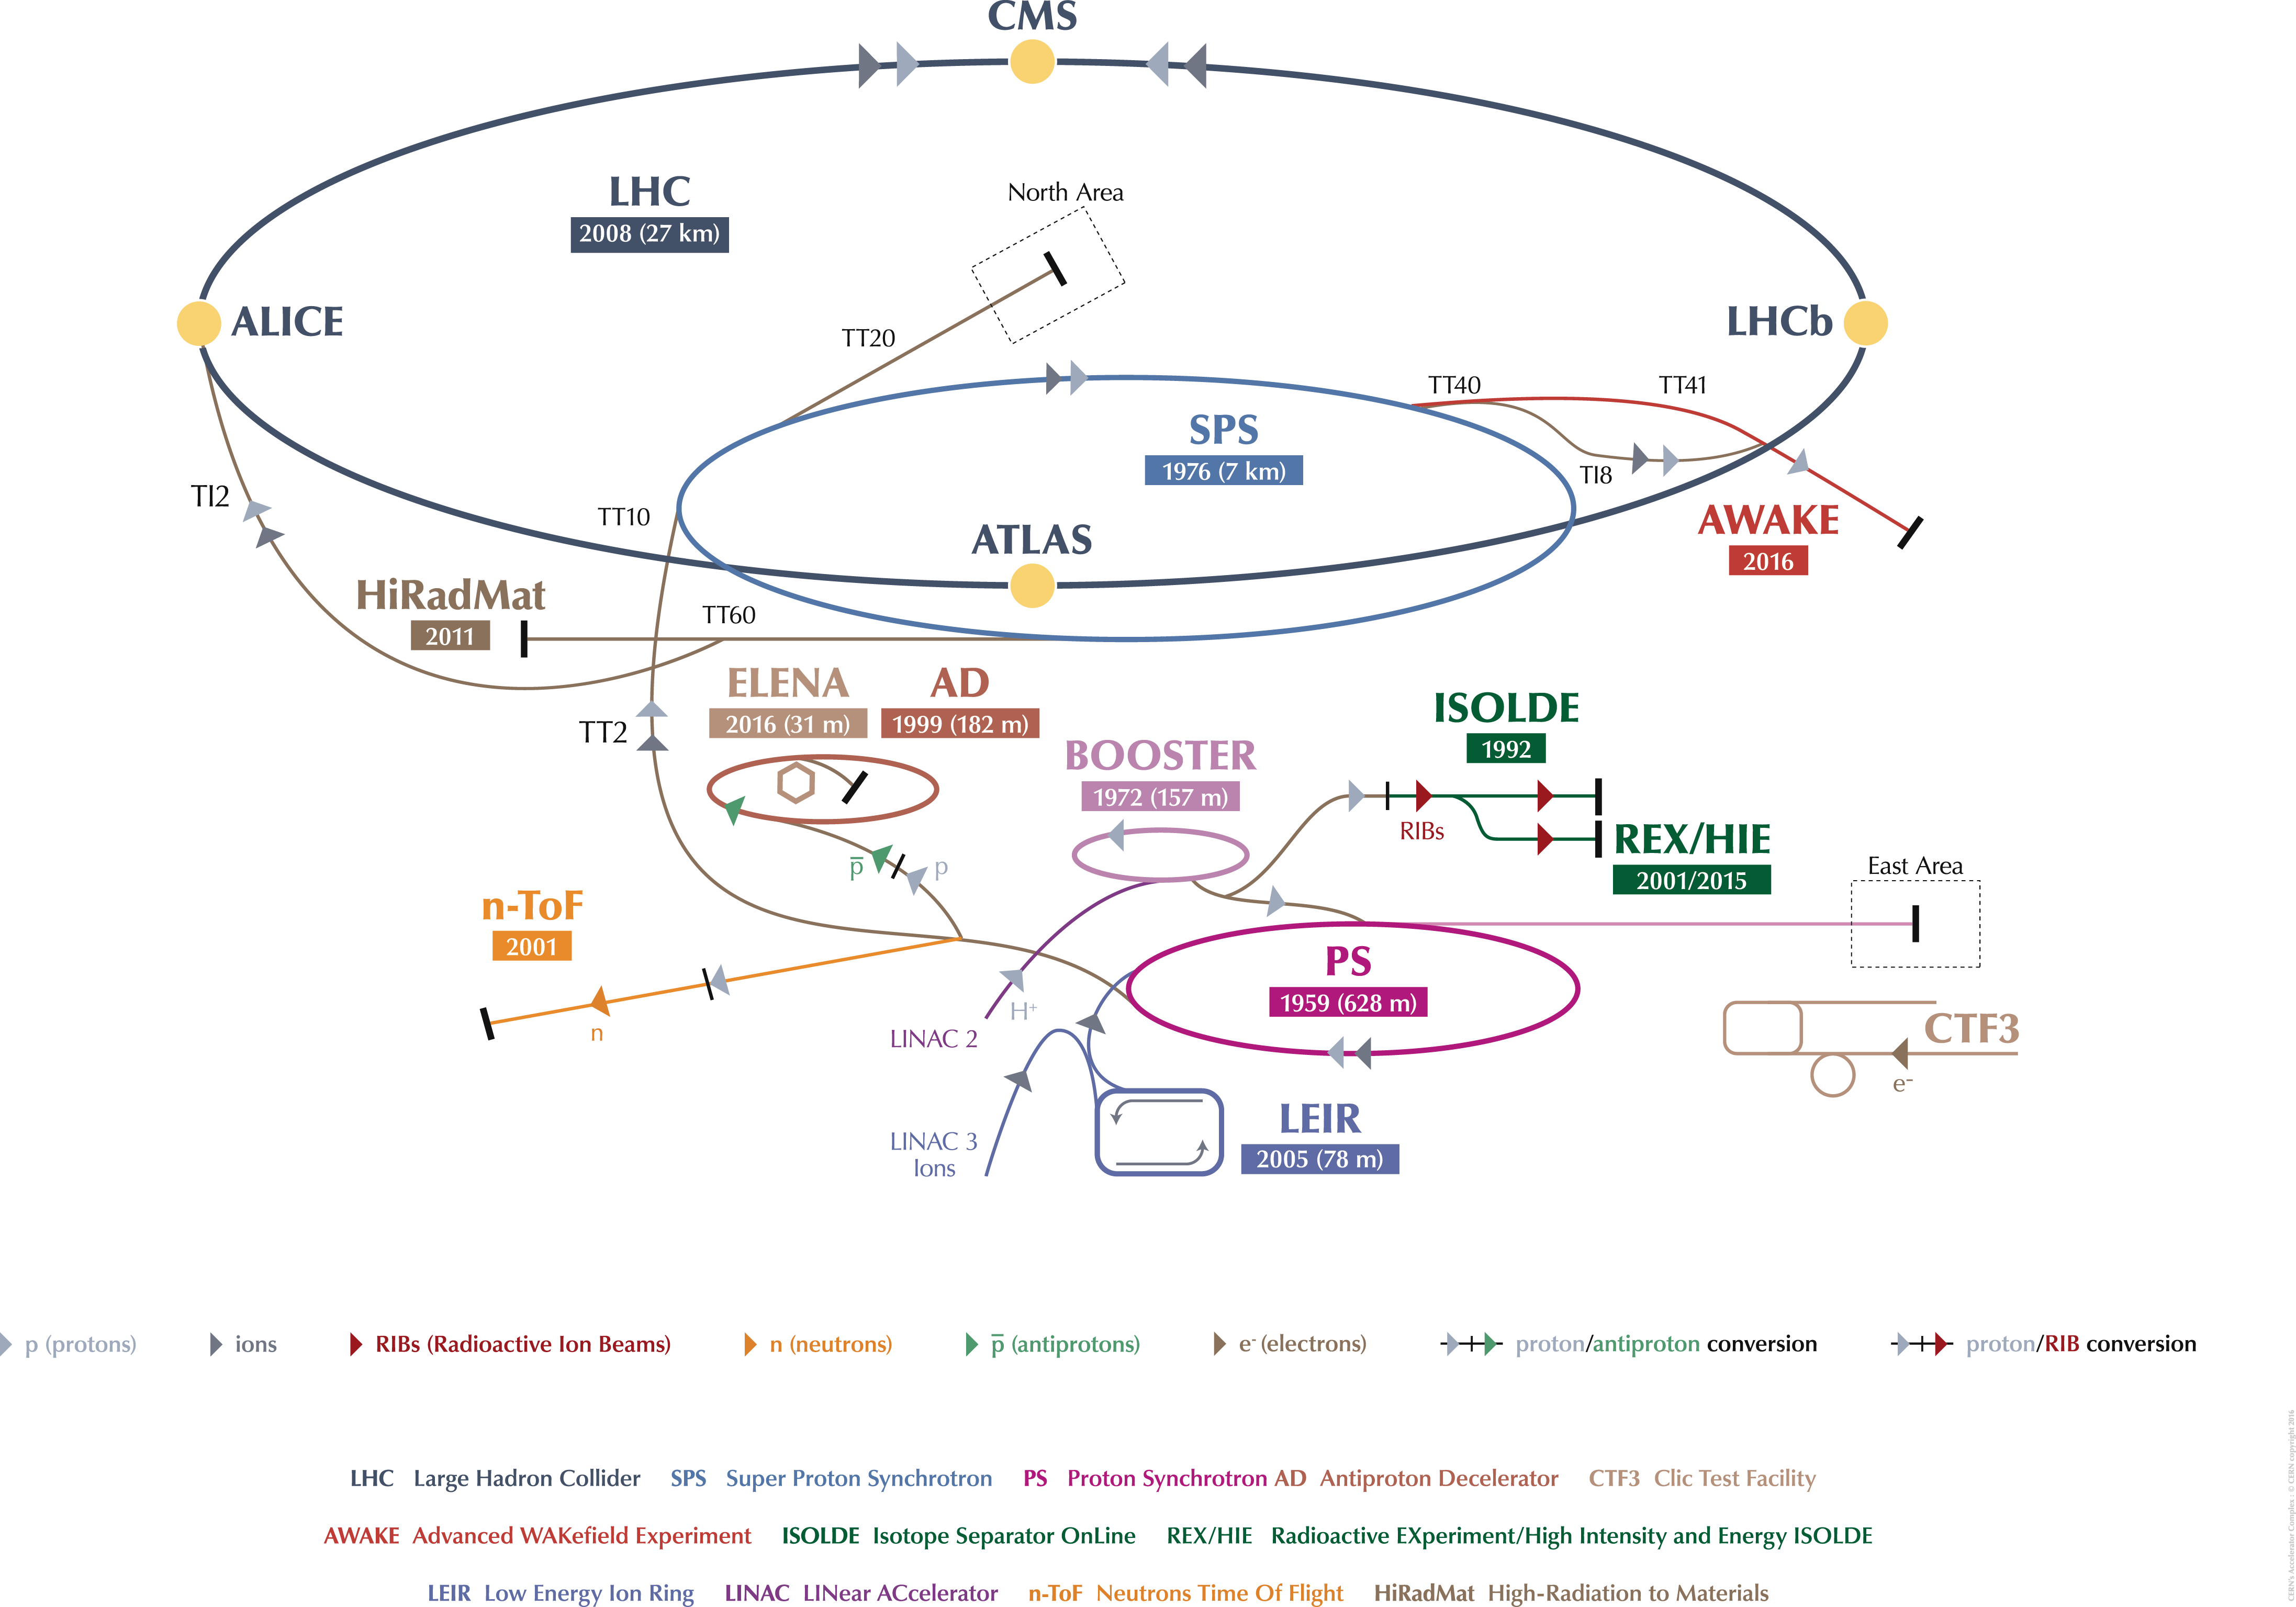
\includegraphics[scale=0.3]{LHC/complexe.png}
  \caption{Schéma du complexe d'accélération du CERN. La chaine d'injection du LHC est constituée du Linac 2, du Booster, du PS et du SPS}
  \label{complexe}
\end{figure}
